
\clearpage
\section{Question 3}

Develop a Simulink model of the circuit shown in Fig. 1(a) using conventional Simulink blocks (i.e., summers, gains, integrals, etc.). Compute the transient response (solutions) on time interval $[0, 0.1]$~s using the ode3 solver with 0.1~ms time-step size.

\subsection*{Block Diagram}
The following block diagram represents the Simulink implementation of the RLC circuit for part (a):
\begin{figure}[H]
	\centering
	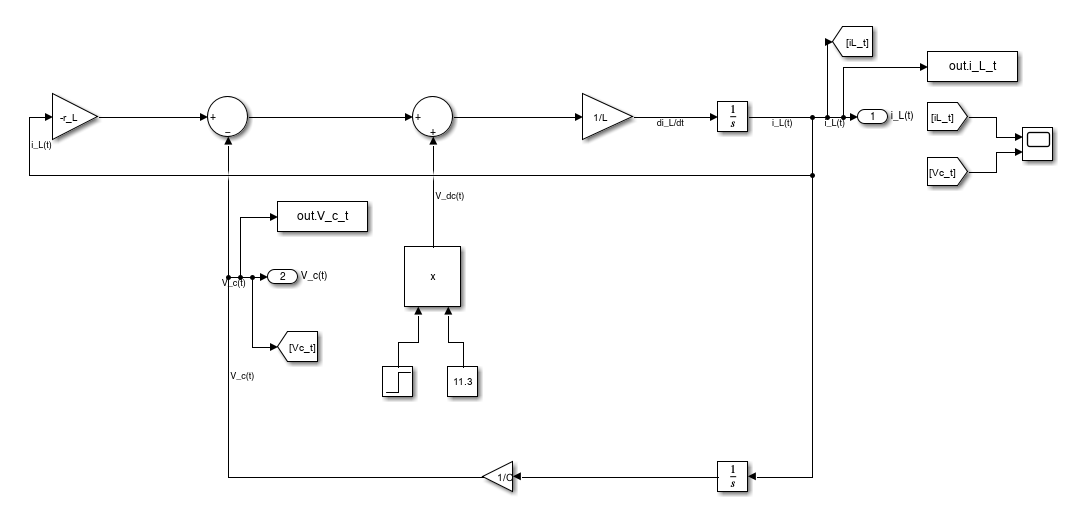
\includegraphics[width=0.85\textwidth]{figures/hw01_q03_block-diagram-RLC-circuit.png}
	\caption{Simulink block diagram for the series RLC circuit (part a).}
\end{figure}

\subsection*{Simulation Results}
The transient response of the circuit was simulated in Simulink using the \texttt{ode3} solver with a fixed time step of 0.1~ms over the interval $[0, 0.1]$~s. The following plot shows the inductor current $i_L(t)$ and capacitor voltage $v_C(t)$:
\begin{figure}[H]
	\centering
	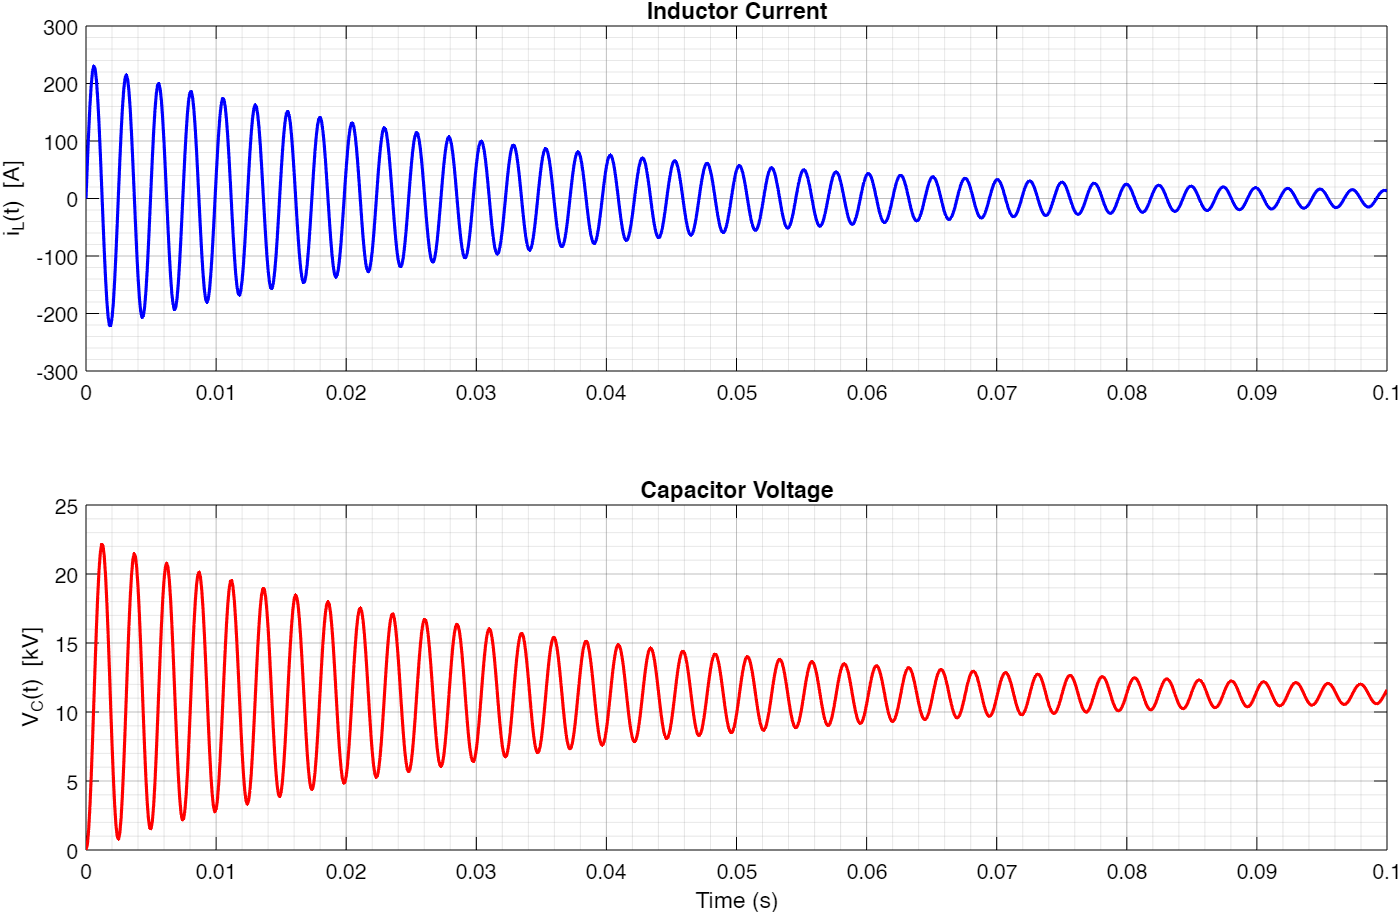
\includegraphics[width=0.85\textwidth]{figures/hw01_q03_plot-of-iL-and-Vc.png}
	\caption{Simulink simulation results: $i_L(t)$ and $v_C(t)$ for the RLC circuit.}
\end{figure}

\subsection*{Discussion}
The simulation results show the expected underdamped oscillatory response, consistent with the analytical solution derived in Q1 and Q2. The current and voltage waveforms exhibit oscillations with a slow decay, as predicted by the low damping ratio ($\zeta = 0.0104$). The Simulink model accurately captures the circuit dynamics using only basic blocks and the specified solver settings.
